\definecolor{lightgray}{rgb}{.9,.9,.9}
\definecolor{darkgray}{rgb}{.4,.4,.4}
\definecolor{purple}{rgb}{0.65, 0.12, 0.82}

\lstdefinelanguage{JavaScript}{
  keywords={typeof, new, true, false, catch, function, return, null, catch, switch, var, if, in, while, do, else, case, break},
  keywordstyle=\color{blue}\bfseries,
  ndkeywords={class, export, boolean, throw, implements, import, this},
  ndkeywordstyle=\color{darkgray}\bfseries,
  identifierstyle=\color{black},
  sensitive=false,
  comment=[l]{//},
  morecomment=[s]{/*}{*/},
  commentstyle=\color{purple}\ttfamily,
  stringstyle=\color{red}\ttfamily,
  morestring=[b]',
  morestring=[b]"
}

\lstset{
   language=JavaScript,
   backgroundcolor=\color{lightgray},
   extendedchars=true,
   basicstyle=\footnotesize\ttfamily,
   showstringspaces=false,
   showspaces=false,
   numbers=left,
   numberstyle=\footnotesize,
   numbersep=9pt,
   tabsize=2,
   breaklines=true,
   showtabs=false,
   captionpos=b
}

\hypersetup{
    colorlinks=true,
    linkcolor=blue,
    filecolor=magenta,      
    urlcolor=blue,
}
\urlstyle{same}

\nnarticleheader{A ‘Spin’ on Modeling Propeller Movement}{Kieran Dias-Lalcaca, Elijah Lee, and Ryan Ngo, Haverford '20}
\noindent
\textbf{Introduction}

Propellers have revolutionized the capacity of naval and aeronautical transportation, energy, and dozens of other fields. The idea of being able to propel oneself or some medium through space and time has intrigued us since the Egyptians and Archimedes figured out how to use a screw to lift water out of a river. Thus this technology was revolutionary and is critical to our modern world. At first glance, modeling the operation of a propeller appears to be relatively simple. However, upon closer investigation, one will realize that the behavior of a propeller requires deeper investigation into different axes and dimensions. Using sinusoidal functions, we can model the movement of a propeller as it moves through time. This relationship allows for an inquiry into how sinusoidal functions operate in three dimensions and the relationship between modeling and real-world solutions.

\noindent
\textbf{Breaking it Down}

To start thinking about how we could model a propeller, we decided to break it up into more manageable pieces to figure out the many problems individually. Firstly, we thought of one blade of the propeller rotating on a fixed axis at a fixed forward speed. This limited the number of variables that we had to worry about, but still allowed us to figure out how a system of this complexity would operate mathematically. We decided that GeoGebra was the best way to model this function as Desmos would only allow us to operate in two dimensions. 

With our parameters set and our assumptions noted, we set to work trying to figure out how a sinusoidal function would be used as a model for a propeller. Starting with a general cosine function, as it was decided that it made more sense to start from one extremity or the other rather than in the middle of a rotation, we began to manipulate and play with the different aspects of a sinusoidal function. The amplitude was, somewhat arbitrarily, set as 10 units as the length of the propeller blade should not affect the overall mathematical function. This can be justified due to the fact that because this model for a perfect physics world, without air resistance, torque, or any other of the thousands of other forces that are present in the real world, a purely mathematical model would not change (other than in amplitude, which we want to change). From there we set a period of \(2\pi\), again just as a hypothetical value that would be easy to work with, and then came to the conclusion that all other vertical and phase shifts are negligible. Thus, we had the model of one blade spinning through time and space in one axis, and therefore we could have as many models of propeller blades spinning through time and space in one axis as we wanted by copying our formula. 

This, however, presented the real challenge; despite how many models we wanted to make of one blade spinning through space and time in one axis, we needed to make a model that had multiple blades spinning through space and time in 3 axes. Therefore, we needed to make a system that could model the blades in 3 dimensions. Thus, we arrive at the second stage of thinking in our breakdown of thought, which is the ability to have a 3D model of a blade spinning through space. We eventually came to the idea of a system of functions to define our curve in 3D space.

Within GeoGebra, we made use of the Curve command, which essentially acts as a wrapper for a three function system.
\begin{figure}[ht]
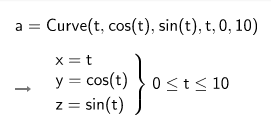
\includegraphics{system.png}
\caption{A screenshot from GeoGebra, showing the breakdown of the Curve command.}
\label{fig:system}
\end{figure}

Looking at Figure \ref{fig:system}, we can start to see the structure of the Curve command. The first three parameters define the x, y, and z functions for the curve. Any transformations we want to apply to the curve must be applied to both sinusoidal functions defining the curve. The next parameter specifies the variable, and the last two specify the start and end of the curve (the domain). Using this command, we can easily begin to define our general formula.

This breakdown, described by our general formula, was the result of a lot of trial and error, research with external sources, and much creative thought on how to be able to combine these individual functions effectively.

\noindent
\textbf{General Formula}

Using these realizations, we were able to create a generalized formula/procedure for generating the parameters of the sinusoidal parameters of the curve command in GeoGebra.
For future reference:
\begin{center}
\(\omega\) = angular frequency\\
RPS = rotations per second\\
RPM = rotations per minute\\
\(l\) = number of blades\\
\(t\) = time\\
\(c\) = horizontal shift\\
\(p\) = period
\end{center}

The next step was to determine each of the values which factored into propeller motion. In order to create a model, we used three values: blade length, rotation speed, and number of blades.

We first started with blade length. Because the blades are rotating around an axis, the length is equivalent to the amplitude of any sinusoidal functions. 

Next, we needed to incorporate rotation speed. Rotations are defined in RPMs, or rotations per minute. In our case, one rotation is equivalent to one period. Thus, changing the rotation speed changes the length of one period. In order to use this information, we first have to convert RPMs into RPS (rotations per second). Our time axis is in seconds, so we need our time units to be in seconds as well. 
\[\frac{x\mbox{ rotations}}{1\mbox{ minute}}\cdot\frac{1\mbox{ minute}}{60\mbox{ seconds}}=\frac{x}{60}\mbox{ rotations per second}\]

Next, we can use this information to find the period of our functions. The period is defined as the time for the function to complete one full cycle, or one rotation. We start with rotations per second and we are looking for the time to complete a cycle; in other words, we are looking for seconds (time) per rotations (cycles). The reciprocal of our RPS gives us our period.
\[p=\frac{1}{\mbox{RPS}}\]

Lastly, we have to convert our period into our angular frequency. We can ask: How many times does our function repeat (cycles, or periods) in the same amount of time as the parent function (\(2\pi\))? Here is the equation we can use:
\[\omega=\frac{2\pi}{p}\]

For example, let's say we have a rotation speed of 30 RPMs. First, we start by converting 30 RPM to RPS.
\[\frac{30\mbox{ rotations}}{1\mbox{ minute}}\cdot\frac{1\mbox{ minute}}{60\mbox{ seconds}}=\frac{30}{60}\mbox{ rotations per second}=0.5\mbox{ RPS}\]
Next, we find our period.
\[p=\frac{1}{0.5}=2\]
Finally, we can find our angular frequency. 
\[\omega=\frac{2\pi}{2}=\pi\]

After rotation speed, we needed to factor in the number of blades. This is a little more complex. Depending on the number of blades, the number of curves changes, which requires each curve’s horizontal shift to change. After finding the period of each curve, we can calculate the shift for each curve. 

For explanation, assume a two blade propeller with a period of \(2\pi\). The two curves need to be equally spaced from each other. In other words, the peaks of the second curve needs to land in between the peaks of the first. We can visualize this in Desmos (Figure \ref{fig:desmos1}). Shifting the second function by \(\frac{1}{2}\) of the period moves it halfway between the first function’s starting point and the next period. \(\frac{2\pi}{2}=\pi\)

We can modify this reasoning to fit situations with more blades. Generalizing our findings, we can say that the distance between each curve should be \(\frac{p}{l}\). From our previous example:
\[\frac{2\pi}{2\mbox{ blades}}=\pi\]
Another example, keeping our period 2pi but with three blades (Figure \ref{fig:desmos2}):
\[\frac{2\pi}{3\mbox{ blades}}=\frac{2}{3}\pi\]
Therefore, the second blade should be shifted \(\frac{2}{3}\pi\) from the first, and the third shifted \(\frac{4}{3}\pi\) from the first (\(\frac{2}{3}\) from the second blade). By multiplying our shift between each blade by the blade number - 1, we get the total shift from the first blade for the given blade. Combining these two findings, we can say that:
\[c_n=\frac{p}{l}\cdot(n - 1)\]
where \(n\) is the 1st, 2nd,...nth blade.

\begin{figure}[ht]
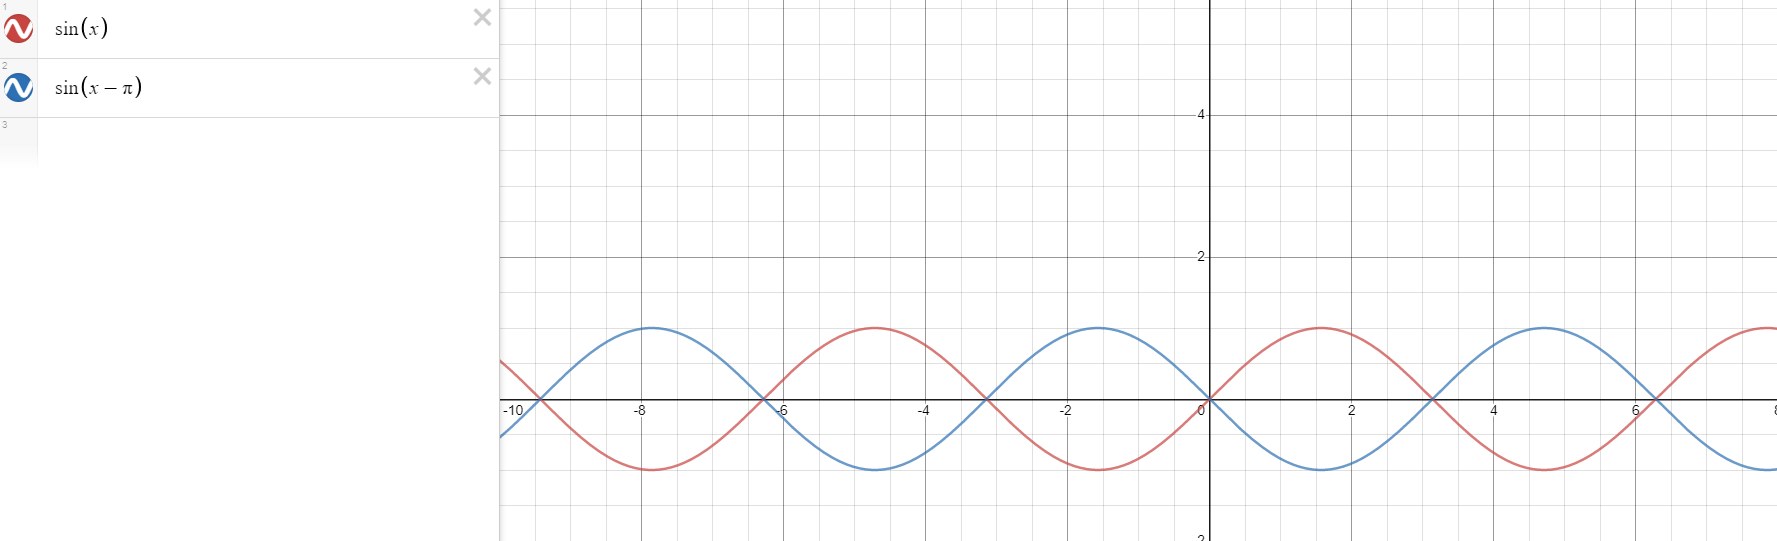
\includegraphics[width=\linewidth]{desmos1.png}
\caption{Desmos graph, showing the proper spacing for two waves}
\label{fig:desmos1}
\end{figure}

\begin{figure}[ht]
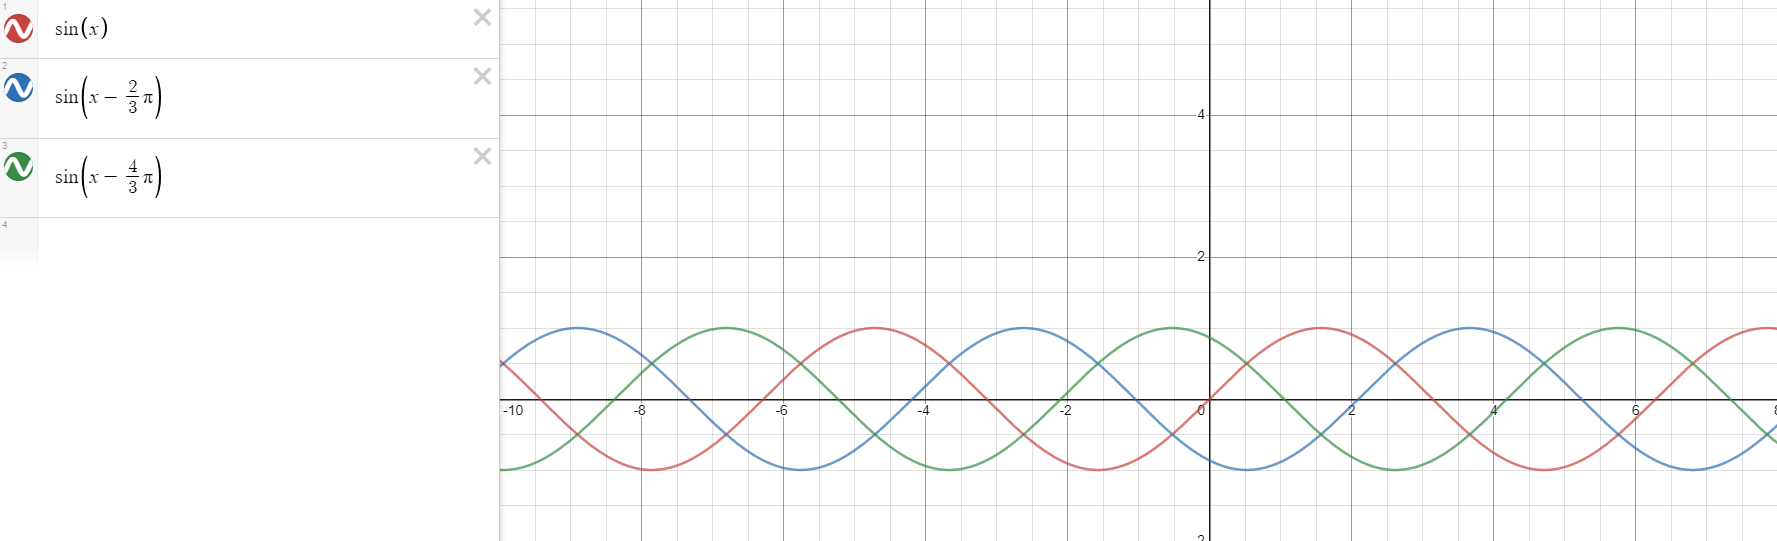
\includegraphics[width=\linewidth]{desmos2.png}
\caption{Desmos graph, showing the proper spacing for three waves}
\label{fig:desmos2}
\end{figure}

Finally, the Curve command requires a start time and end time. Because we are using time as our independent variable, we can start our function at \(t = 0\). The end time is left to the user to define. By leaving the end time up to the user, we can better visualize the movement of the propeller as it moves through time.

Though the equation at first seemed complicated to dive into, after defining each part, it was now only a matter of what type of propeller we wanted to focus on and plugging in values.

\noindent
\textbf{Real-life Application}

In order to use our model to simulate a real-life situation, we found a video of a glass-bottomed boat. \href{https://www.youtube.com/watch?v=EdXxg20XguY}{YouTube Video}

We found a portion of the video where the propeller reached its maximum speed. The video was listed at 30 frames per seconds. By advancing frame-by-frame for thirty frames, we counted two total rotations. The frame rate is 30 FPS; so the propeller had 2 rotations per every thirty frames, or one second. The propeller has three blades (\(l=3\)). 

In order to plot the movement of this propeller, we had to determine its four values. 

First is blade length. While we could not definitively measure the blade diameter from the video due to a lack of scale, this value is not crucial to the other calculations, only affecting the size of the spirals. We chose to leave the blade length as 1. 

Second, we determined the angular frequency from the propeller speed. Using our method from our general formula:
\[\omega=\frac{2\pi}{\frac{1}{RPS}}\Rightarrow\omega=\frac{2\pi}{\frac{1}{2}}\Rightarrow\omega=4\pi\]
\[\therefore p=\frac{2\pi}{4\pi}=\frac{1}{2}\]

Third, we determined the horizontal shift for each curve. According to our formula:
\[c_n=\frac{p}{l}\cdot(n - 1)\]
where \(n\) is the 1st, 2nd,...nth blade.\\
1st blade:
\[c_1=\frac{\frac{1}{2}}{3}\cdot(1-1)=0\]
2nd blade:
\[c_2=\frac{\frac{1}{2}}{3}\cdot(2-1)=\frac{2}{3}\]
3rd blade:
\[c_3=\frac{\frac{1}{2}}{3}\cdot(3-1)=\frac{4}{3}\]

Lastly, we used a slider to represent the end time. By using a slider, we can “scroll” through the simulation and see the propeller locations at any time.

Putting all these arguments together yields three curve functions.
Click this link to see the fully plotted example in GeoGebra. By manipulating the v slider, you can change the end point of the graph.
\url{https://www.geogebra.org/classic/m9z6frdr}

\noindent
\textbf{Going Further}

Using the aforementioned general formula, we wanted to create a fully customizable and parameterized simulation. By utilizing the scripting feature within GeoGebra, we were able to fully integrate the steps needed to generate our functions straight into our GeoGebra project. Figure \ref{fig:simuex1} shows an example use of the capabilities of our simulation.
\begin{figure}[ht]
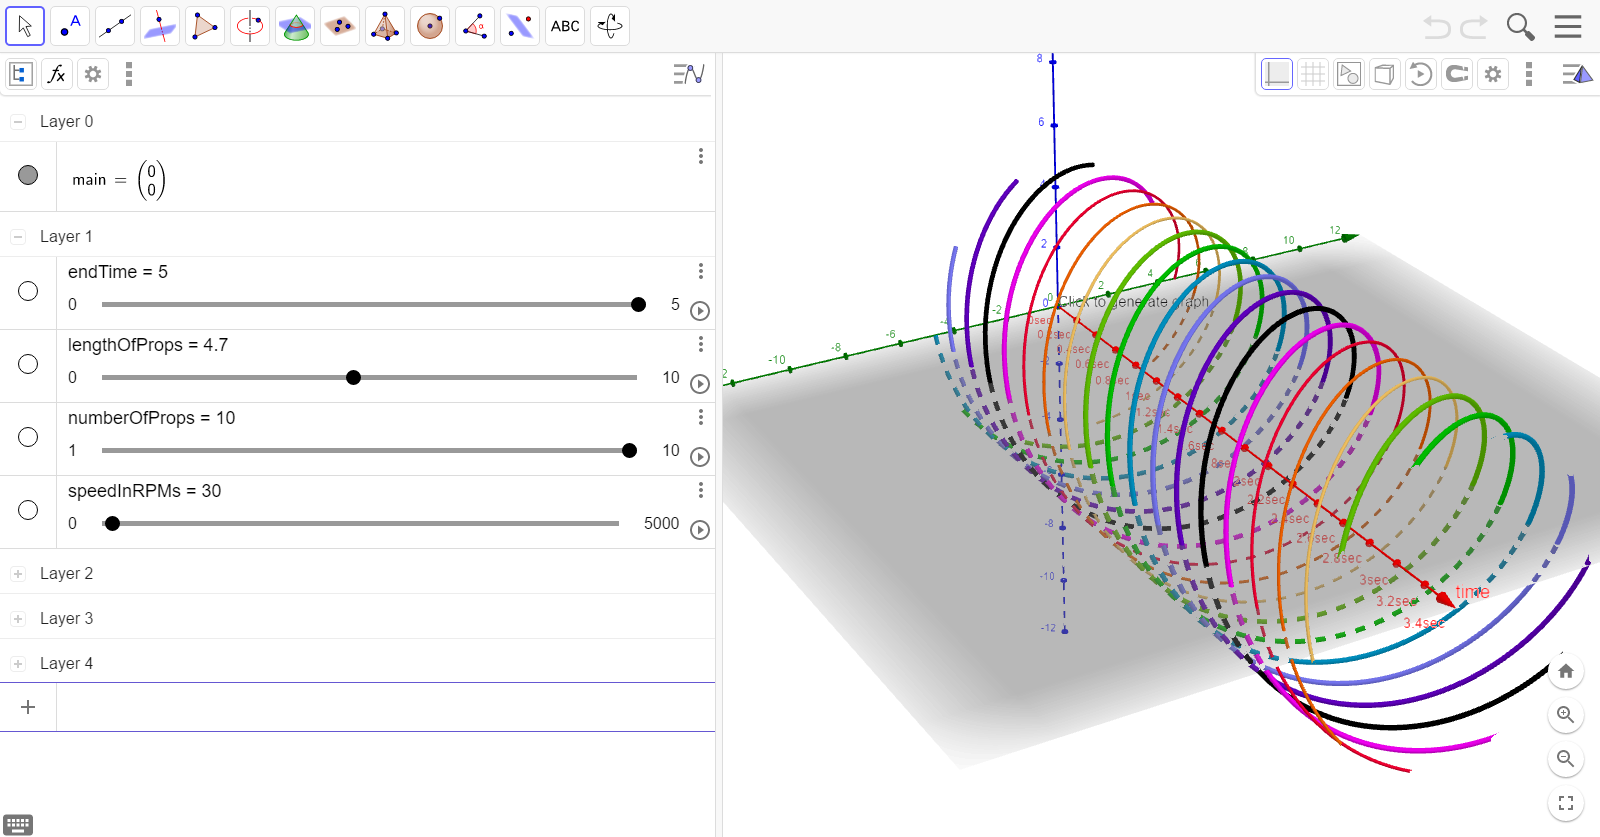
\includegraphics[width=\linewidth]{simuex.png}
\caption{An example simulation.}
\label{fig:simuex1}
\end{figure}

Click this link to access our fully scripted and parameterized simulation: \url{https://www.geogebra.org/classic/y4d4kaua}

\noindent
\textbf{Simulation Explanation}

Layer 0 contains a “main” object, centered at the origin. This object handles the main calculations for the simulation. Each time parameters are edited, clicking on this object recalculates the simulation.
Listing \ref{lst:jscode} shows a cleaned version of the JavaScript behind the main object. This script controls the visibility of objects, angular frequency, and each function's horizontal shift.
\begin{lstlisting}[caption={JavaScript attached to main object},label={lst:jscode},captionpos=b]
// Setup inputs
var numProps = ggbApplet.getValue("numberOfProps");
var speedRPM = ggbApplet.getValue("speedInRPMs");
var amp = ggbApplet.getValue("lengthOfProps");
var end = ggbApplet.getValue("endTime");


// Hide all spiral objects
for (var i = 97; i <= 106; i++) {
    ggbApplet.setVisible(String.fromCharCode(i)+String.fromCharCode(i), false);
}

// Show number needed
for (var i = 97; i <= 97 + (numProps - 1); i++) {
    ggbApplet.setVisible(String.fromCharCode(i)+String.fromCharCode(i), true);
}

// Calculate angular frequency
var rps = speedRPM / 60;
angFreq = (2 * Math.PI) / (1 / rps);
ggbApplet.setValue("ang", angFreq);

// Generate spiral offsets
for (var i = 0; i < numProps; i++) {
    var shiftName = String.fromCharCode(i + 97) + "shift";
    ggbApplet.setValue(shiftName, ((1 / rps) / numProps) * i);
}

\end{lstlisting}

Working through Listing \ref{lst:jscode}:

Lines 1-5 grab values from the input slider and assign them to local variables for later use. Next, the script hides each of the curve functions. Lines 8-10 loops through the letters a-j, and hides the correspondingly named objects. The script then shows the necessary number of objects in a similar fashion (lines 13-16). Lines 18-21 calculates the global angular frequency, and outputs the value back into an object. Lastly, lines 23-27 generate the horizontal shift for each function, following the general formula.

Layer 1 contains all of the parameters. You can use the sliders or directly input desired values into the fields. Each time an edit is made, click on the main point to recalculate the simulation.

Layer 2 holds all of the curve functions. This simulation supports a maximum of ten propellers; thus, there are ten curve functions. GeoGebra scripting does not support the creation of new objects. Therefore, it is easiest to pre-create objects and activate them as needed. To avoid using reserved letters (e, i, etc.), function names are doubled up. Using this function as an example:
\[\mbox{aa}=\mbox{Curve}(t, \mbox{amp}\cdot\cos(\mbox{ang}(t-\mbox{ashift})), \\ \mbox{amp}\cdot\sin(\mbox{ang}(t-\mbox{ashift})), t, 0, \mbox{endTime})\]

We are using the Curve command built in to GeoGebra, as before. The parameters remain identical. However, there are additional elements to the sinusoidal functions.
\[\mbox{amp}\cdot\cos(\mbox{ang}(t-\mbox{ashift}))\]
amp is a variable linked to the propeller length parameter. It represents the amplitude of the sinusoid, and is identical for each curve.

ang represents the angular frequency. It is linked to the propeller speed parameter. Using the same method from the general formula, RPMs are converted into rotations per second, which is then used to calculate the angular frequency. This value is also equivalent for all of the curves.

ashift represents the horizontal shift of the sinusoid. Each curve has a different horizontal shift; the script calculates each shift using the method in the general formula and then sets the appropriate variable in Layer 3 to its corresponding value. Layer 3 contains all of the shift variables. Layer 4 contains the amplitude variable, and the angular velocity variable.

\noindent
\textbf{Summary}

In closing, we found an efficient and concise process to properly model propeller movement. Through the investigation process, we had many realizations about the behavior of sinusoids. In addition, the complexity of modeling a function in three dimensions allowed us to dig deeper not only into sinusoids, but also in defining a function in 3D space. Using GeoGebra allowed us to visualize the changes we made, and see how changes to different parts of our function affected the 3D spiral in different ways. As we investigated, we encountered many different situations which prompted further investigation. Especially when investigating the new three dimensional space, many “side investigations” took place to help explain “why?”. We think that our model is an accurate representation of real-life conditions. However, studies have found that real-life movement deviates from models. As seen in Figure \ref{fig:real}, actual propeller movement varies slightly from the modeled theoretical path. Despite this inconsistency, our model still provides an accurate depiction of ideal propeller movement.

\begin{figure}[h]
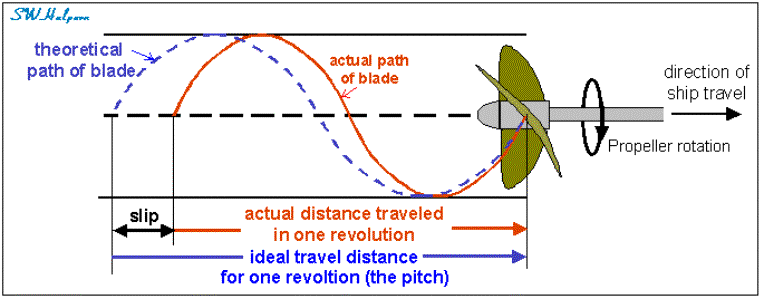
\includegraphics[width=\linewidth]{image019.png}
\caption{Diagram comparing the ideal theorized movement of a propeller vs. actual movement. (Source: www.titanicology.com/)}
\label{fig:real}
\end{figure}

Our goal was to provide the viewer with a simple simulation of propeller movement through time. Through this simple simulation, it is clear that propeller movement is just one of many examples of sinusoids in our world. After all, Da Vinci once said, “Simplicity is the ultimate sophistication.”